%%&program=xelatex
%&encoding=UTF-8 Unicode
% SVN keywords
% $Author: bernardo $
% $Date: 2014-10-24 15:26:00 +0100 (Fri, 24 Oct 2014) $
% $Revision: 6732 $
% $URL: http://metis.ipfn.ist.utl.pt/svn/cdaq/Users/Bernardo/Aulas/LFEB/teXfiles/ContrucoesGeometrica/ConstrucoesGeomet.tex $
\documentclass[a4paper,12pt]{article}      % Comments after  % are ignored
%\usepackage{hyperref}                 % For creating hyperlinks in cross references
%
%MUDAR procedimento lente divergente + angulo de Brewster
\usepackage{ifxetex}% for XELATEX, or PDFlatex
\usepackage{ifplatform} 
%
\ifxetex
	\usepackage{polyglossia} \setmainlanguage{portuges}
	\usepackage{fontspec}
	\ifwindows
		\setmainfont[Ligatures=TeX]{Garamond}
		\setsansfont[Ligatures=TeX]{Gill Sans MT}
		\setmonofont{Consolas}		
%		\setmonofont[Scale=MatchLowercase]{Courier}
	\fi
	\iflinux
		\setmainfont[Ligatures=TeX]{Linux Libertine O}
		\setsansfont[Ligatures=TeX,Scale=MatchLowercase]{Linux Biolinum}
		\setmonofont[Scale=MatchLowercase]{Courier}
	\fi
	\ifmacosx
	% add settings
	% Use xelatex -no-shell ...
		\setmainfont[Ligatures=TeX]{Garamond}
		\setsansfont[Ligatures=TeX]{Helvetica}
		\setmonofont{Consolas}
	\fi
	\usepackage{xcolor,graphicx} 
\else
	\usepackage[portuguese]{babel}
	%\usepackage[latin1]{inputenc}
	\usepackage[utf8]{inputenc}
	\usepackage[T1]{fontenc}
	\usepackage{graphics}                 % Packages to allow inclusion of graphics
	\usepackage{color}                    % For creating coloured text and background
\fi

\usepackage{enumitem}
\setlist{nolistsep}

\usepackage{tikz}
%\usetikzlibrary{calc,arrows,decorations.pathmorphing,intersections}


\usepackage{amsmath,amssymb,amsfonts} % Typical maths resource packages
\usepackage[retainorgcmds]{IEEEtrantools}

\oddsidemargin 0cm
\evensidemargin 0cm

\pagestyle{myheadings}         % Option to put page headers
                               % Needed \documentclass[a4paper,twoside]{article}

\markboth{{MEFT}}
{{\small\it \protect\input{../../LIFE.txt}}}

\addtolength{\hoffset}{-0.5cm}
\addtolength{\textwidth}{2.5cm}
\addtolength{\topmargin}{-1.5cm}
\addtolength{\textheight}{3cm}

%\textwidth 15.5cm
%\topmargin -1.5cm
\setlength{\parindent}{0pt}
\setlength{\parskip}{1ex  plus  0.5ex  minus  0.2ex}
%\parindent 0.5cm
%\textheight 25cm
%\parskip 1mm


% Math macros
\newcommand{\ud}{\,\mathrm{d}} 
\newcommand{\HRule}{\rule{\linewidth}{0.5mm}}

\author{Prof. Bernardo B. Carvalho} 

%%%%, Bernardo Brotas Carvalho\\bernardo@ipfn.ist.utl.pt} 
\date{ Outubro 2012} 

\begin{document} 

	
\includegraphics[width=0.2\textwidth]{../../logo-ist}%\\[1cm]  %%  Logo_IST_color

	\HRule \\[0.5cm]
	{ \huge \sf  \textsc{Instrumentos Ópticos Simples e \\ Goniómetro}} \\[0.4cm] % \bfseries 
%	{ \huge \sf  \textsc{Sistemas ótipos baseados em Lentes Delgadas e aproximação paraxial} }\\[0.4cm] % \bfseries 
%	{ \large \bfseries Construções Geométricas em Lentes Delgadas %(aproximação paraxial)}\\
%	{ \large \bfseries Procedimento Experimental}\\
	\HRule \\%[0.5cm]

%\newpage
\section{\sf Introdução}
Pretende-se com este trabalho desenhar e montar no laboratório montagens ou sistemas ópticos compostos com duas ou mais lentes delgadas, testando as suas características principais. As duas montagens -- um telescópio simples e um microscópio -- são variações do esquema óptico apresentado na Secção 5 do Trabalho de Óptica Geométrica. 

Nestes sistemas, designamos por \emph{objetiva} a lente que está do lado do objeto e por \emph{ocular} aquela que está do lado do observador, com distâncias focais $f_{obj}$ e $f_{ocu}$ respetivamente. Em ambos os casos, a ocular está  próxima da \emph{imagem intermédia} A'B' formada pela objetiva. Sendo a distância inferior à distância focal $f_{ocu}$, a imagem final será \emph{virtual}, ou seja, visível apenas através da lente.\footnote{Cf. \emph{Guia de Óptica Geométrica}, Secção 3.5.}
Assim, o papel da ocular consiste em ampliar a imagem intermédia, tal como um lupa amplia um objeto.
 Continua-se neste trabalho a usar a análise da óptica geométrica paraxial ou de 1.ª ordem.


Como segundo objetivo, pretende-se que os alunos tomem conhecimento e aprendam a manusear e a tomar medidas corretamente  com um instrumento óptico de precisão, o \emph{goniómetro}. Este instrumento permite medir ângulos de desvio, por reflexão ou refração de feixes de raios paralelos, com uma resolução inferior a um minuto de grau.

\subsection{\sf O olho humano}

\begin{figure}
	[!htb]  \centering 
	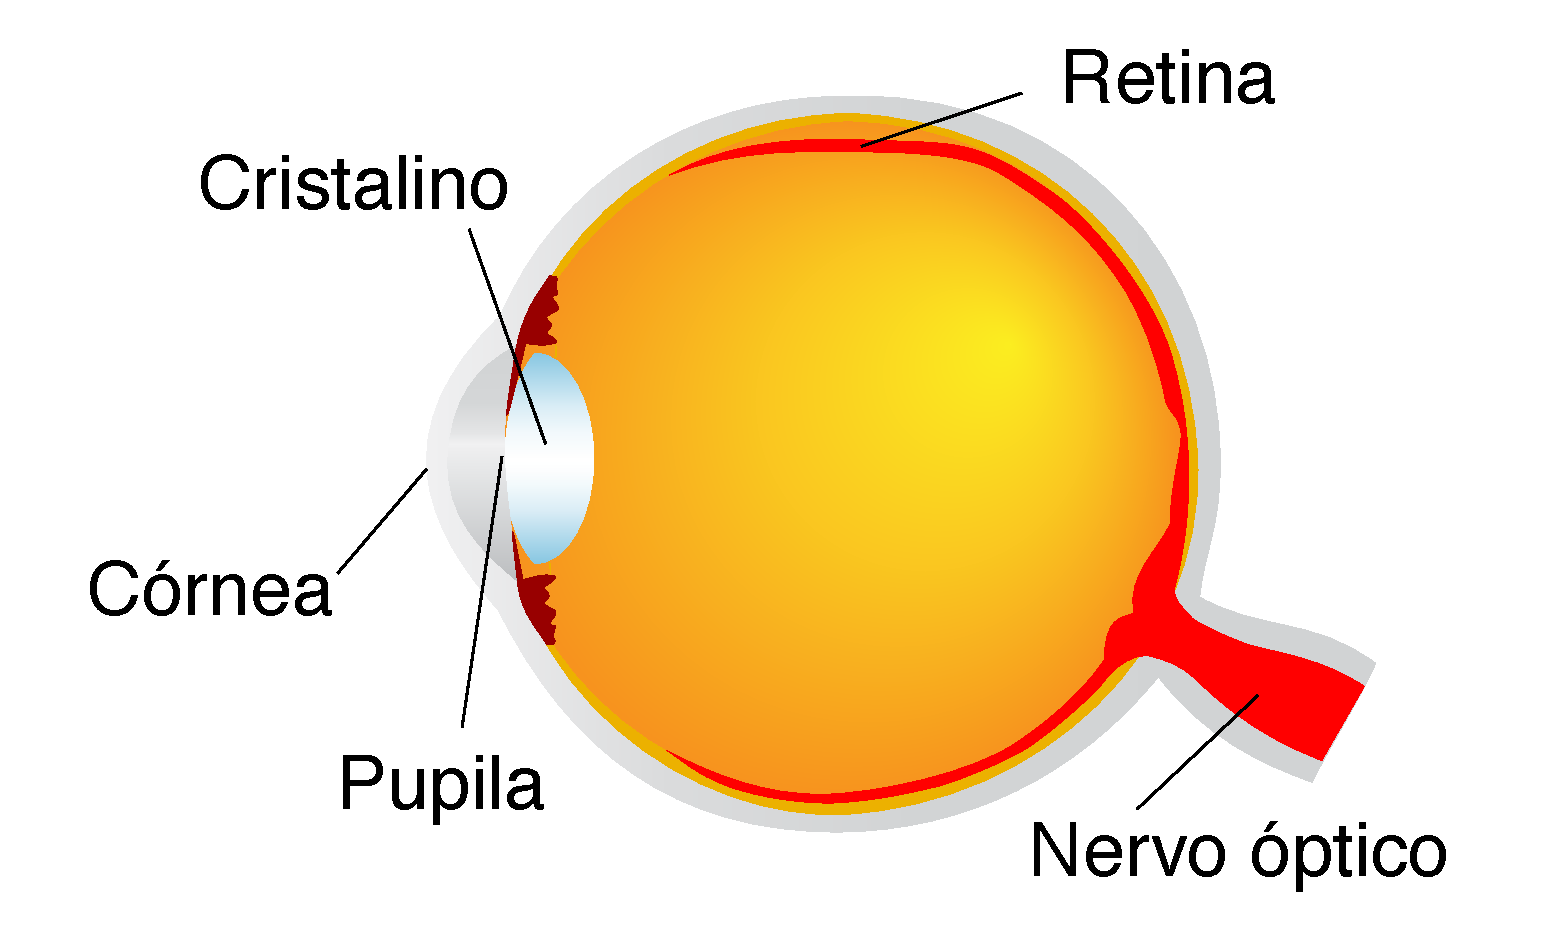
\includegraphics[width=0.6\textwidth]{olho-1}
	\caption{Diagrama dos principais elementos do olho humano. \label{fig:olho-1}} 
\end{figure}

Para efeitos práticos, considera-se o infinito óptico qualquer distância superior a 5 m. Para o nosso estudo, a lente da córnea e a lente do cristalino são substituídas por um sistema equivalente constituído por uma única lente, com o máximo de distância focal $f$ igual a 2,5 cm, que é a média da distância entre a córnea e a retina (Fig. \ref{fig:olho-1}). A potência em dioptrias (dt) desta lente equivalente é dada por:

\begin{equation}
D=\frac{1}{f} \,[\mathrm{m}^{-1}] = \frac{1}{0,025} \,[\mathrm{m}^{-1}] = 40 \,[\mathrm{m}^{-1}]=40\, \mathrm{dt}.
\end{equation}



Se um objecto está no infinito, os raios ópticos vindos dele chegam paralelos ao olho, e são focados na retina sem necessidade de acomodação do olho, ou seja, com o olho relaxado (Fig. \ref{fig:olho-2} à esq.). À medida que o objecto se aproxima do olho é necessário os músculos ciliares aumentarem a curvatura da lente para criar uma imagem focada na retina -- a isto chama-se \emph{acomodação do olho}. O ponto mais próximo do olho para o qual a lente ainda consegue focar a imagem na retina é designado por \emph{ponto próximo} (Fig. \ref{fig:olho-2} à dir.). Esta distância aumenta com a idade e considera-se o ponto próximo igual a 0,25 m para uma visão normal padrão.

\begin{figure}
	[!htb]  \centering 
	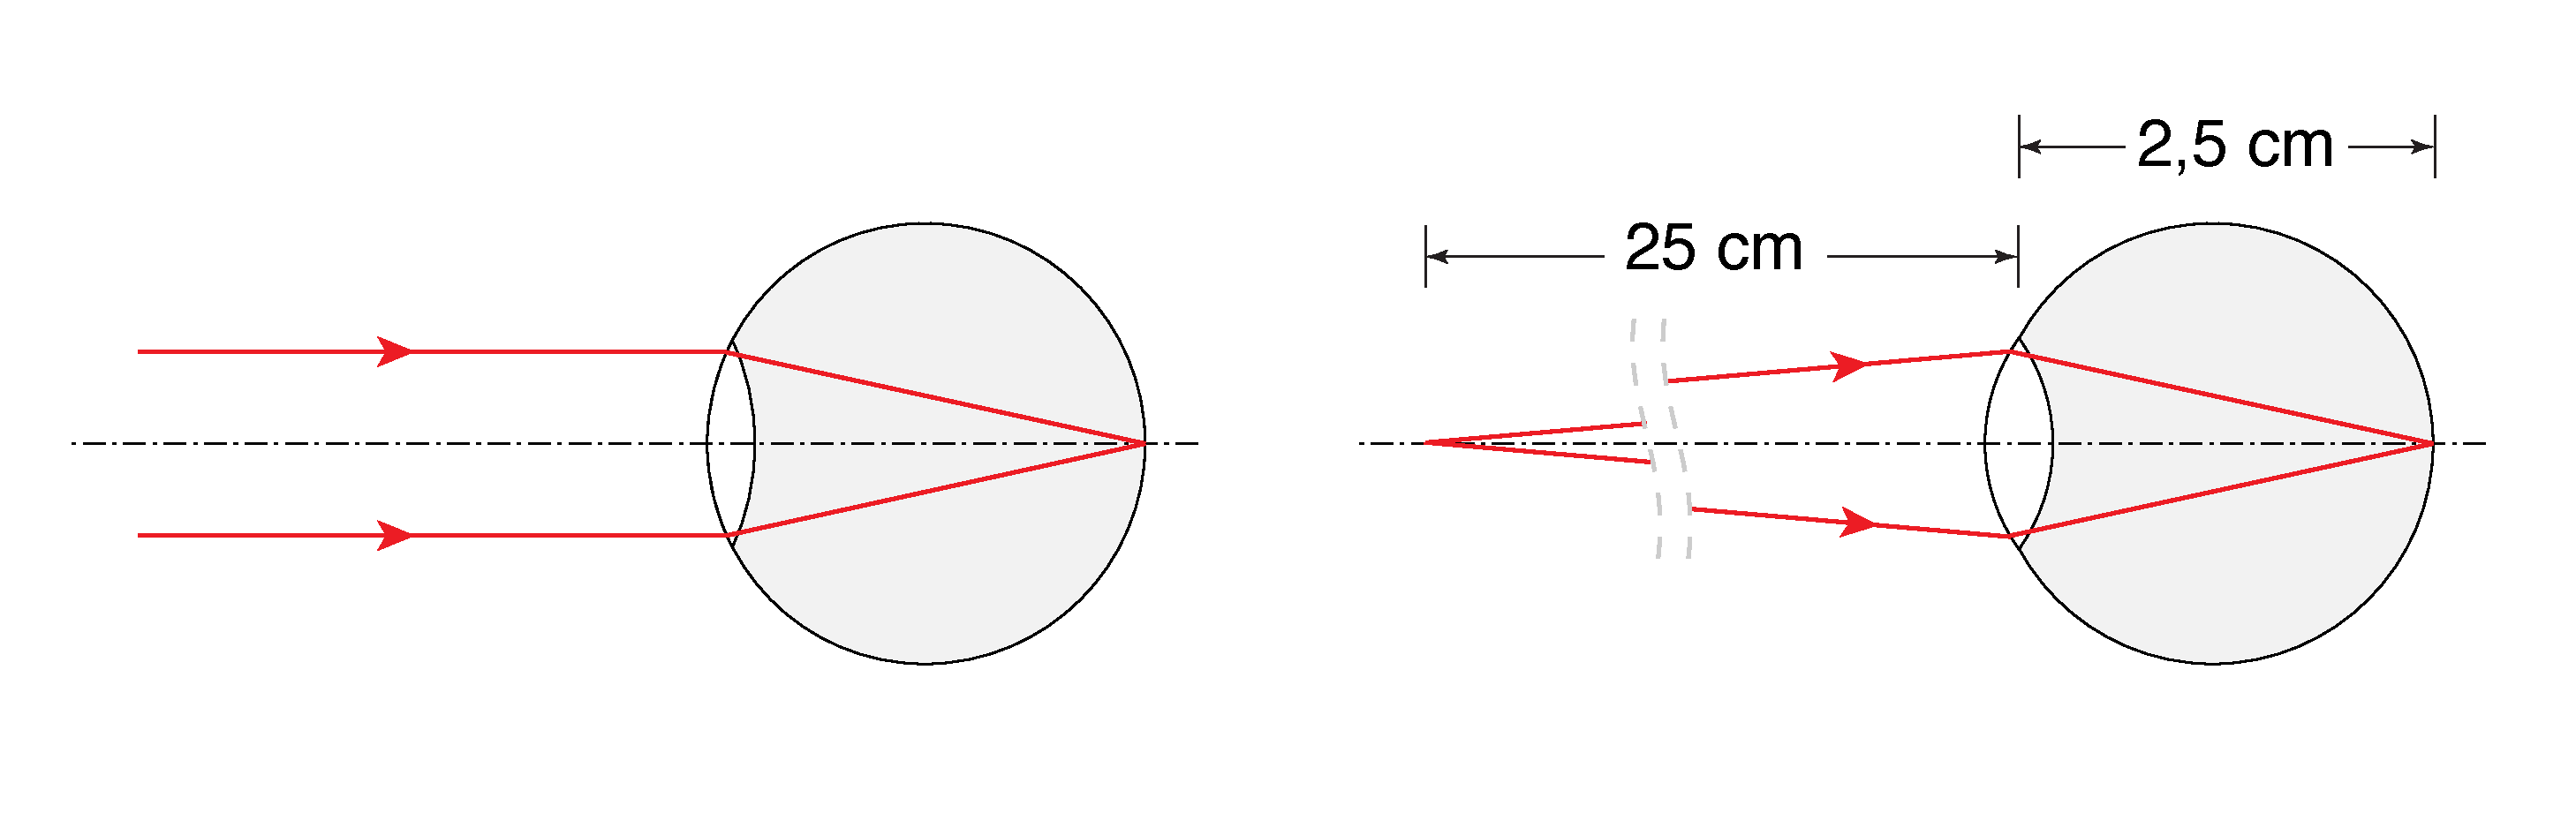
\includegraphics[width=1.0\textwidth]{olho-2}
	\caption{Esquema do olho no caso de objectos no infinito (esq.) e no ponto próximo (dir.). \label{fig:olho-2}} 
\end{figure}
\begin{figure}
	[!htb]  \centering 
	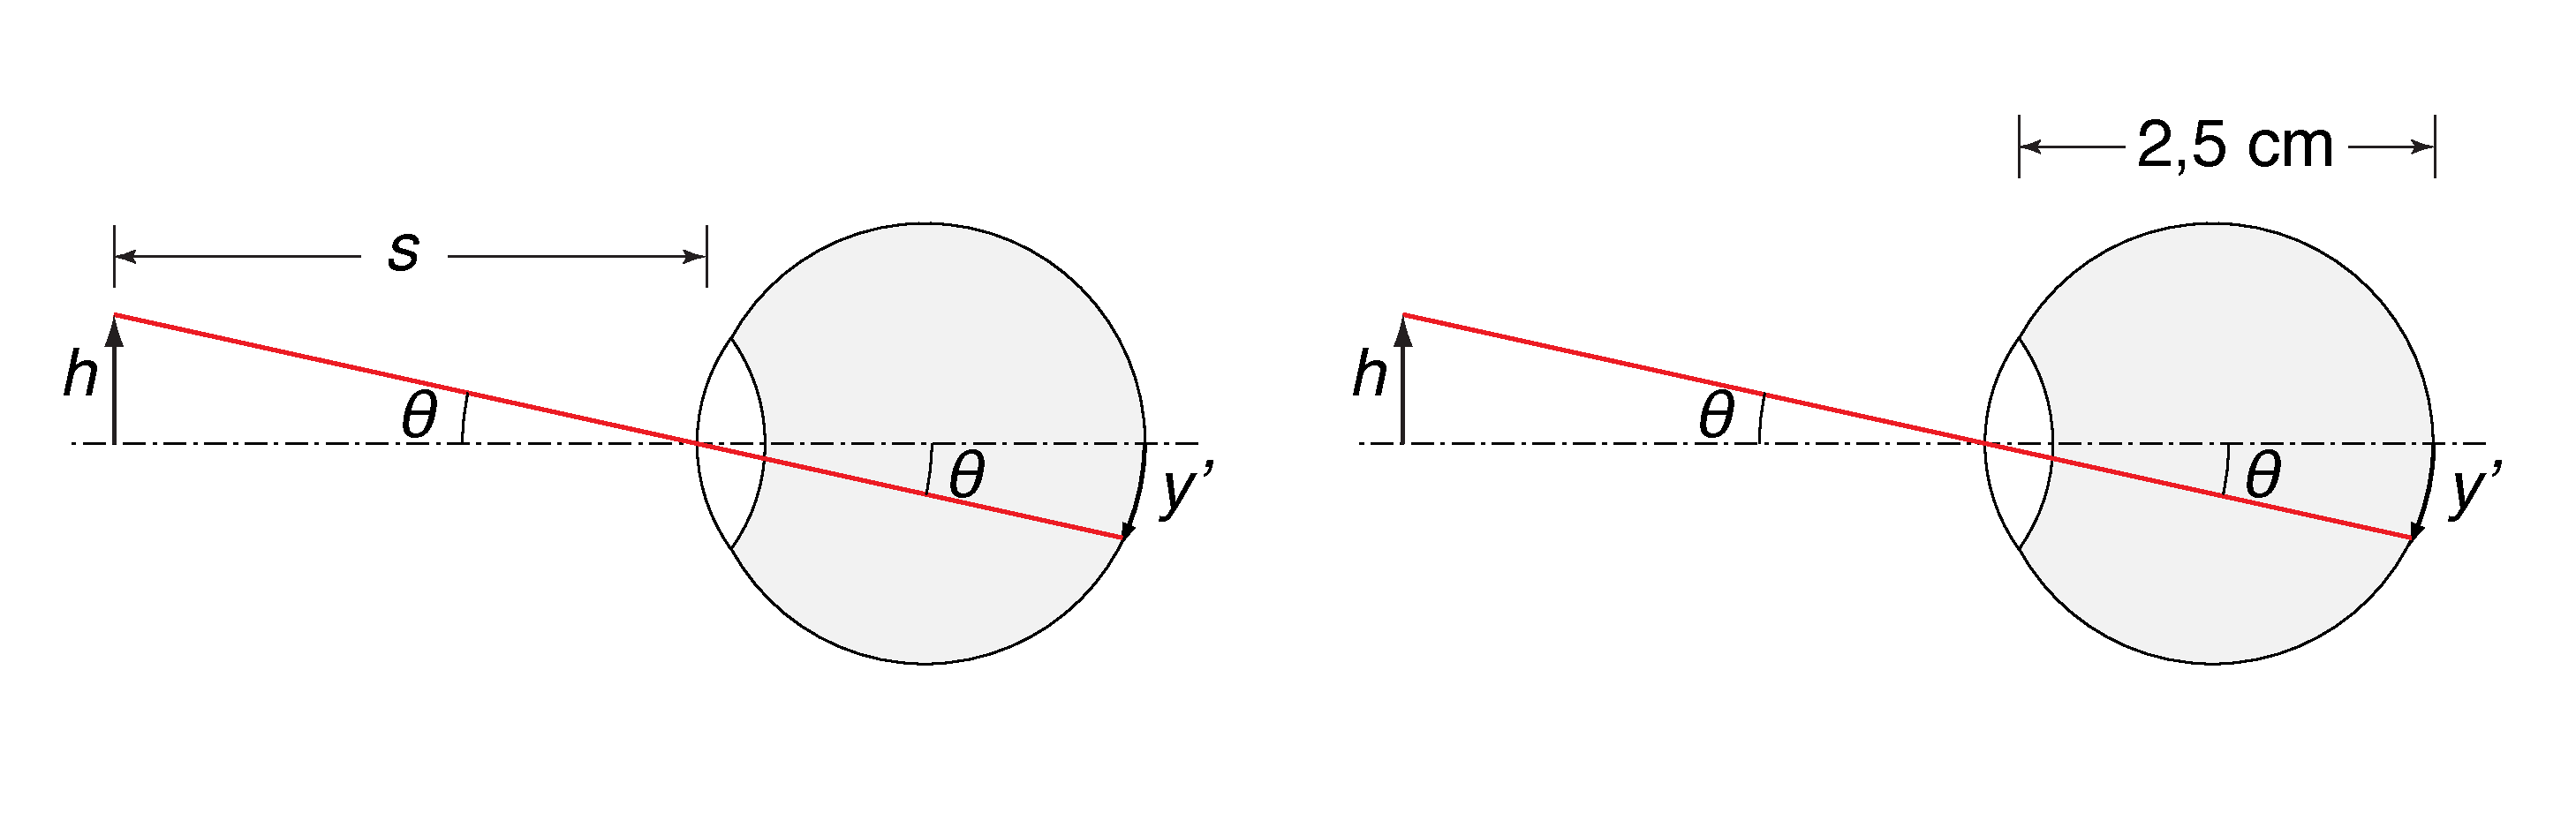
\includegraphics[width=1.0\textwidth]{olho-3}
	\caption{Formação de imagem na retina de um objecto de altura $h$ a uma distância $s$. \label{fig:olho-3}} 
\end{figure}

O tamanho aparente dum objecto é determinado pelo tamanho que a imagem apresenta na retina. Mesmo sem variar o tamanho real do objecto, este pode ser visto maior se o aproximarmos do olho, porque o tamanho da sua imagem na retina é maior. A avaliação do tamanho da imagem na retina pode ser feita através da medição do ângulo $\theta$, que corresponde à inclinação dos raios principais do extremo da imagem (Fig. \ref{fig:olho-3}).

Considere-se um objecto com altura $h$ a uma distância $s$ do olho. Para o objeto podemos escrever $\tan\theta=h/s$, e a para a imagem na retina, $y'$ , temos $\tan\theta = y' /$(2,5 cm). Na aproximação paraxial, ou seja de ângulos pequenos, podemos usar $\tan\theta \approx\theta$, e assim $\theta\approx h/s=y'/$(2,5 cm). Desta relação conclui-se que $y'$, tamanho da imagem na retina, é proporcional a $h$, tamanho do objecto, e inversamente proporcional à distância $s$ entre o objecto e o olho.





\subsection{\sf Lupa}

A lupa simples é o instrumento óptico mais elementar. Consiste numa só lente convergente e permite aumentar o tamanho aparente do objecto, ou seja, o tamanho da imagem na retina. Sabendo que a maior imagem que se pode obter dum objecto com o olho desarmado é quando o objecto está no ponto próximo (Fig. \ref{fig:olho-4}), e dado que $y'_0$, tamanho da imagem na retina, é proporcional ao ângulo definido entre a altura do objecto $h_0$ e a sua distância ao olho, pode-se escrever a relação

\begin{equation}
\theta_0=h_0/0,25
\end{equation}

\begin{figure}
	[!htb]  \centering 
	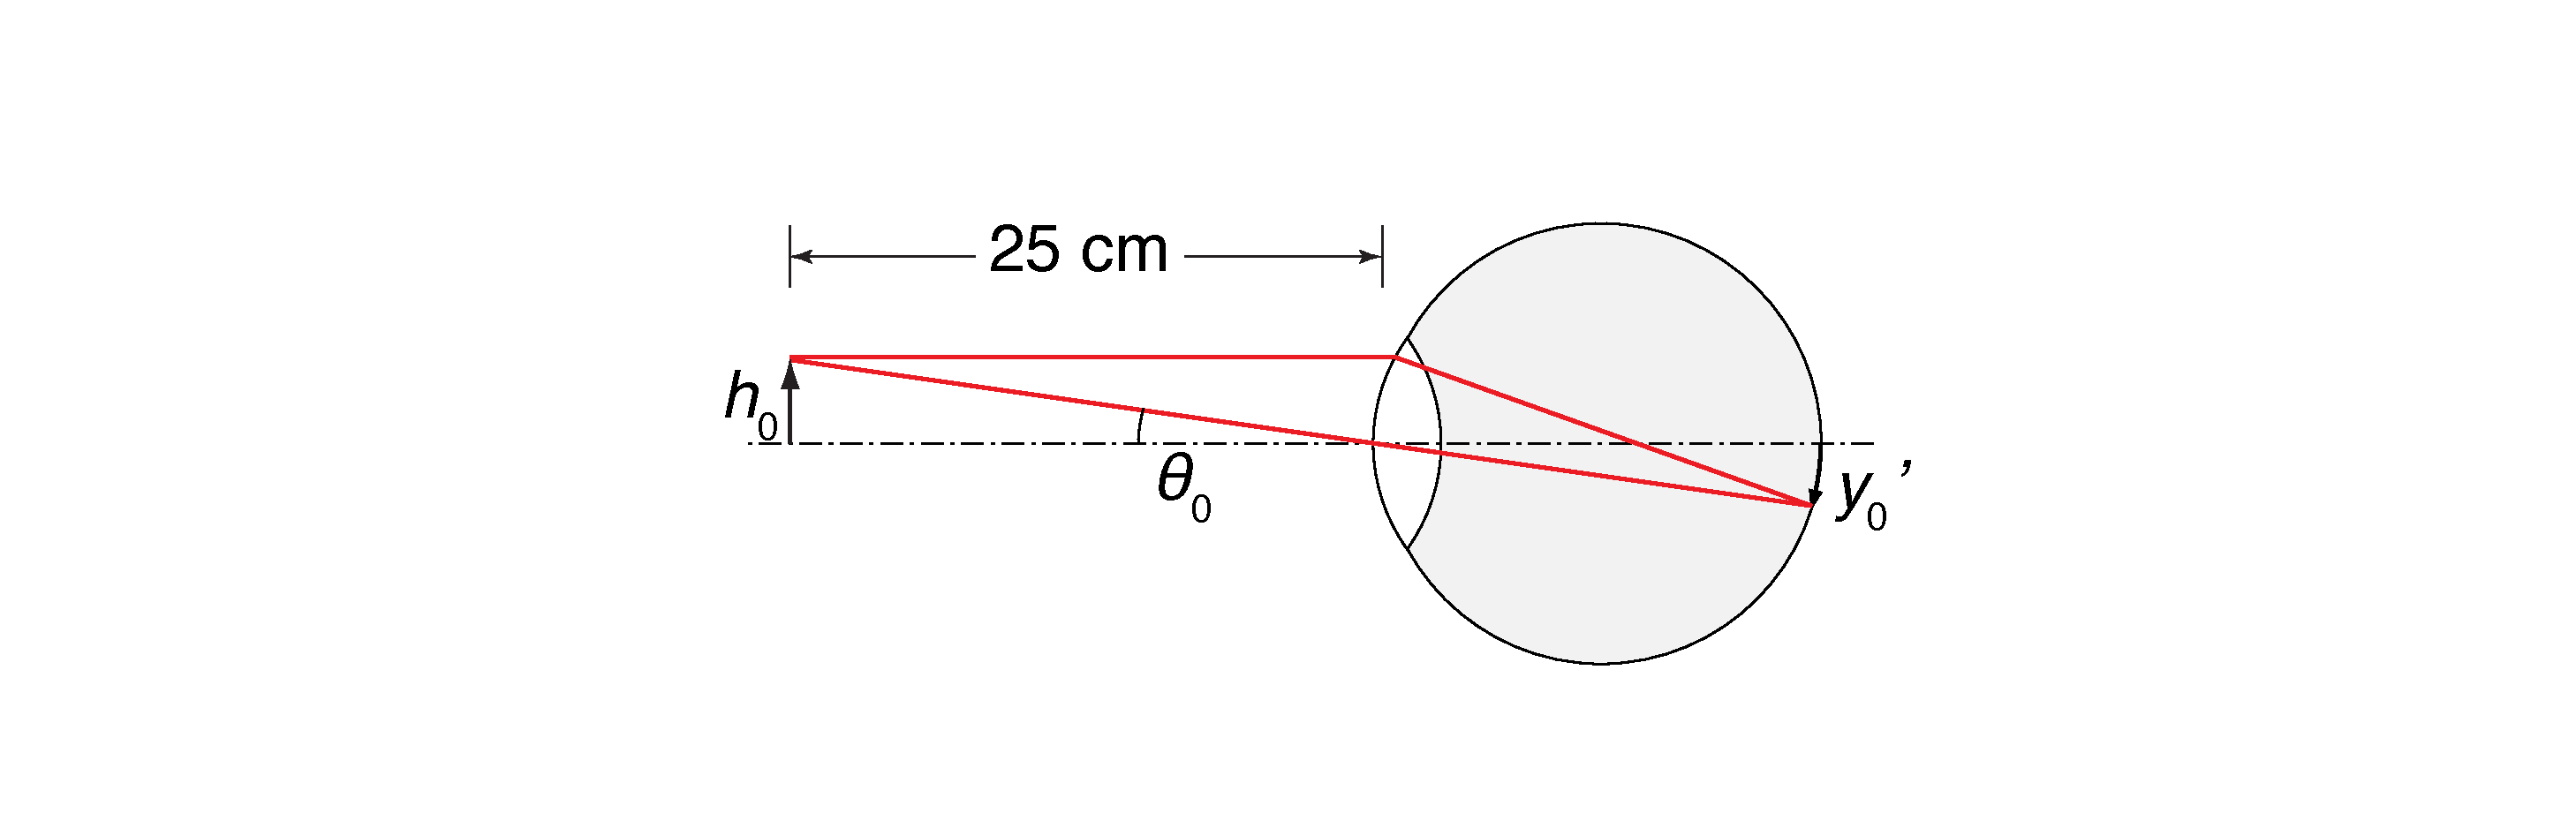
\includegraphics[width=1.0\textwidth]{olho-4}
		\caption{Objecto no ponto próximo visto pelo olho desarmado. \label{fig:olho-4}} 
\end{figure}

Na visão auxiliada pela lupa, esta é colocada perto do olho, e o objecto colocado a uma distância inferior ao foco. A imagem produzida pela lupa é virtual, ampliada e direita.

\begin{figure}
	[!htb]  \centering 
	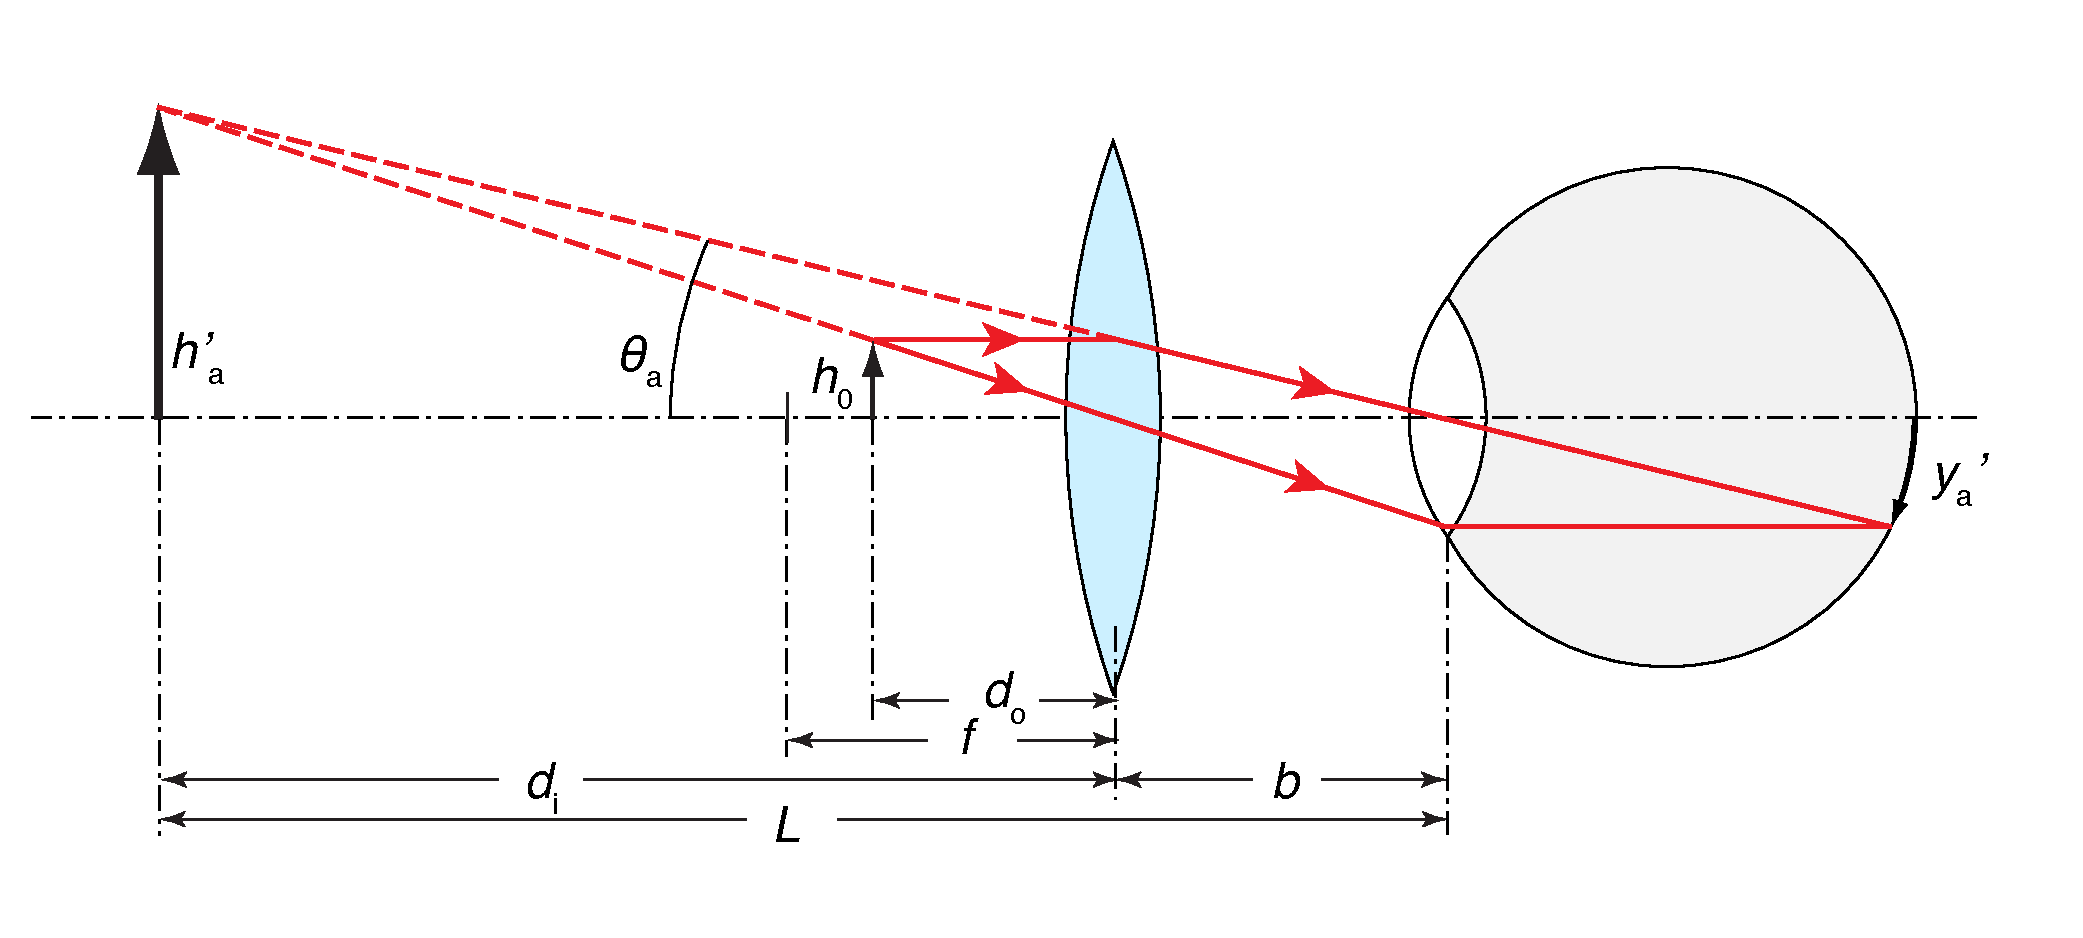
\includegraphics[width=0.8\textwidth]{olho-5}
	\caption{Formação de imagem com o auxílio de uma lupa a uma distância $b$ do olho. O objecto $h_0$ está a uma distância $d_O<f$ da lente, e a imagem (virtual) $h'_a$ aparenta estar a uma distância $d_i$ da lente e $L$ do olho. \label{fig:olho-5}} 
\end{figure}


A \emph{ampliação angular} $M_A$ dum instrumento óptico é determinada pela razão entre $y'_a$, dimensão da imagem na retina quando o objecto é visto através do instrumento (Fig. \ref{fig:olho-5}), e $y'_0$, dimensão da imagem na retina quando vista pelo olho desarmado e o objecto no ponto próximo. Também a razão entre os respectivos ângulos permite esse cálculo, isto é 

\begin{equation}
M_A=\frac{y'_a}{y'_0}=\frac{\theta_a}{\theta_0}
\end{equation}

Tirando partido da aproximação paraxial, temos $\tan\theta_a = h'_a / L \approx \theta_a$ e $\tan\theta_0 = h_0 / 0,25 \approx\theta_0$, portanto pode-se escrever a ampliação angular como:

\begin{equation}
M_A = \frac{h'_a/L}{h_0/0,25}=-\frac{d_i\,0,25}{d_0 L}= \frac{0,25}{L}\left(1-\frac{d_i}{f}\right) 
\end{equation}

onde na última igualdade se recorreu à equação dos focos conjugados. Como a distância à imagem é negativa, $d_i = - (L – b)$, obtém-se por fim

\begin{equation}
M_A = \frac{0,25}{L}\left(1+\frac{L–b}{f}\right)
\end{equation}

Da análise desta expressão pode-se dizer que a ampliação diminui se $L$ ou $b$ aumentam. Existem três casos particulares de ampliação:

\begin{enumerate}

\item  Se $b=f \to M_A = \frac{0,25}{f}$

\item  Se $b=0\to M_A = 0,25\left(\frac{1}{L}+\frac{1}{f}\right)$.
Se $b= 0$ e também $L = 0,25 $ m (valor mínimo para $L$, uma vez que a imagem também deve poder ser focada correctamente pelo olho), então obtém-se para $M_A$ o valor máximo, igual a $M_A = 1+\frac{0,25}{f}$. Este caso corresponde a ter a lupa "encostada" ao olho, e a imagem aumentada surge à distância do ponto próximo.

\item  Se o objecto é colocado no foco ($d_O=f$), então a lupa forma a sua imagem no infinito $(L = \infty)$ e a ampliação é $M_A = \lim_{L\to\infty}\frac{0,25}{L}\left(1+\frac{L–b}{f}\right)= \frac{0,25}{f}$. Neste caso, o olho recebe raios paralelos e não necessita de fazer acomodação, o que é mais cómodo, e a ampliação apenas se reduz de uma unidade relativamente ao caso 2.
\end{enumerate}

%%%%%%%%%%%%%%%%%%%%%%%%%%%%%%%%%%%%%%%%%
\section{\sf Microscópio composto}

O microscópio é o instrumento óptico empregado para observar objectos pequenos, colocados muito próximos do instrumento. Na sua forma mais simples, consiste em duas lentes convergentes. A lente mais próxima do objecto (\emph{objectiva}) tem uma distância focal $f_{obj}$ menor que a distância focal $f_{ocu}$ da lente mais perto do olho (\emph{ocular}) (Fig. \ref{fig:microscopio}).

\begin{figure}
	[!htb]  \centering 
	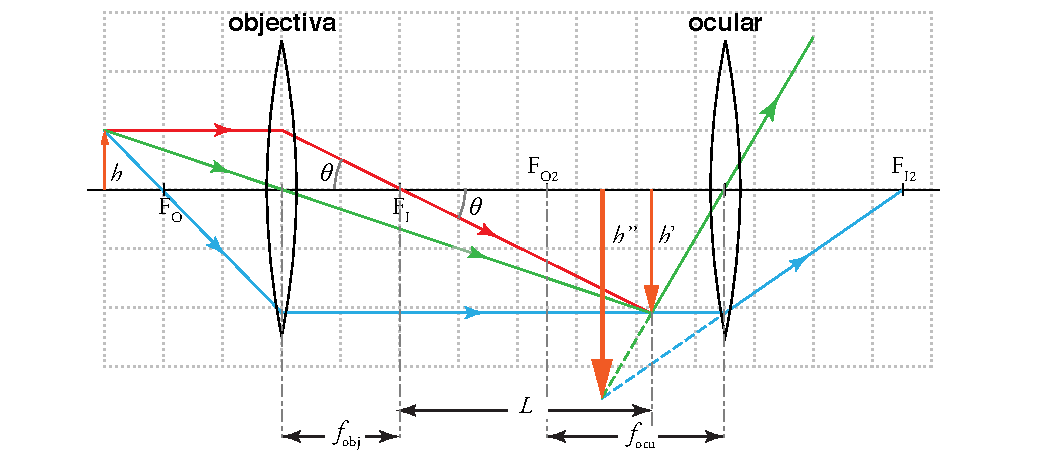
\includegraphics[width=1.0\textwidth]{microscopio}
		\caption{Formação de imagem num microscópio. \label{fig:microscopio}} 
\end{figure}

Um objecto de altura $h$ é colocado, em relação à objectiva, mais afastado do que o foco desta, de modo a produzir uma imagem de tamanho $h'$ que é real, invertida e maior que o objecto. A objectiva produz uma imagem com \emph{ampliação transversal linear} $M_T$, dada por:

\begin{equation}
M_T=\frac{h'}{h} = -\frac{L\tan\theta}{f_{obj}\tan\theta}= -\frac{L}{f_{obj}}
\end{equation}

O sinal negativo indica que a imagem é invertida e, uma vez que é real, a imagem pode ser projectada sobre um alvo para se medir o seu tamanho.

A lente ocular é usada para aumentar a imagem formada pela lente objectiva. Assim, a ocular é colocada de modo a que a imagem $h'$ produzida pela objectiva (agora \emph{objecto virtual} da segunda lente) venha localizar-se a uma distância ligeiramente inferior ao seu foco $f_{ocu}$. Nesta condição, a ocular actua como uma simples lupa, que permite trazer o objecto $h’$ para uma distância mais curta do que o ponto próximo (0,25 m), e produz a imagem $h''$. Esta imagem, maior que o objecto e virtual, pode ser medida com um ecrã transparente.

A \emph{ampliação final} $M$ é dada pelo produto da ampliação linear para a lente objectiva e a ampliação angular obtida para a lente ocular,

\begin{equation}
M = \frac{h''}{h}=M_T\times M_A =\frac{h’}{h}\times\frac{0,25}{f_{ocu}}=-\frac{L}{f_{obj}}\times\frac{0,25}{f_{ocu}}.
\end{equation}


\subsection{\sf Procedimento Experimental}

Material: Lente objectiva $f$ = 75 mm e ocular $f$ = 150 mm.

\begin{enumerate}
\item Na folha quadriculada em anexo desenhe um diagrama de traçado de raios, com o objecto a uma distância do foco igual $\approx f/5$. Obtenha a posição da imagem intermédia e da imagem final.
\item Monte o esquema como indicado na Fig. \ref{fig:microscopio}.
\item Projecte sobre um ecrã a imagem $h’$ claramente focada e meça a sua ampliação.
\item Ajuste a ocular de modo a ver uma nova imagem, $h’’$, focada.
\item Sobre o ecrã transparente visualize a imagem virtual h’’. Foque bem em simultãneo a escala do ecrã e a imagem virtual.
\item Meça a ampliação final e compare com a ampliação teórica.
\end{enumerate}

%%%%%%%%%%%%%%%%%%%%%%%%%%%%%%%%%%%%%%%%
\section {\sf Telescópio}
O telescópio é o instrumento óptico utilizado para observar, em geral, grandes objectos muito afastados do instrumento, procurando trazer a imagem do objecto para mais perto. O tipo de telescópio que vamos construir é composto por duas lentes convergentes: a lente objectiva tem distância focal $f_{obj}$ maior que a distância focal $f_{ocu}$ da lente ocular (Fig. 5).

\begin{figure}
	[!htb]  \centering 
	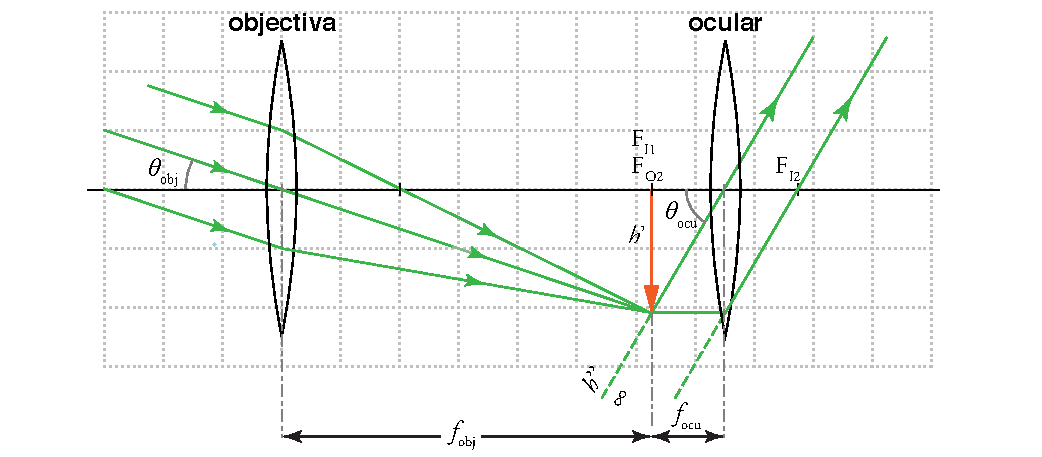
\includegraphics[width=1.0\textwidth]{telescopio2}
		\caption{Formação de imagem num telescópio. \label{fig:telescopio2}} 
\end{figure}

A objectiva vai produzir uma imagem real, invertida e localizada no foco $f_{obj}$, dado que o objecto está no infinito. Esta imagem é muito mais pequena do que o objecto e a finalidade da objectiva não é de aumentar, mas apenas de produzir uma imagem perto do observador que deve coincidir com o foco, $f_{ocu}$ da lente ocular. Assim, as lentes estão separadas de uma distância igual a $f_{obj} + f_{ocu}$.

A ampliação de um telescópio é apenas a ampliação angular dada pela razão do ângulo $\theta_{obj}$ definido pelo objecto e do ângulo $\theta_{ocu}$ definido pela imagem final. Usando a aproximação paraxial e tendo em conta que a imagem é invertida, temos

\begin{equation}
\tan\theta_{obj}= -\frac{h’}{f_{obj}} \approx \theta_{obj} \,\,\,\,\,\,\,\,\,\tan\theta_{ocu} =\frac{h’}{f_{ocu}}\approx\theta_{ocu}
\end{equation}

e portanto a ampliação final é

\begin{equation}
M=M_A =\frac{\theta_{obj}}{\theta_{ocu}}= -\frac{f_{obj}}{f_{ocu}}.
\end{equation}

\subsection{\sf Procedimento Experimental}

Material: Lente objectiva $f$ = 150 mm e ocular $f$ = 75 mm.

\begin{enumerate}
\item Na folha quadriculada em anexo desenhe um diagrama de traçado de raios, utilizando como objectiva a lente mais potente do trabalho de Óptica Geométrica, e considerando o objecto no infinito. Obtenha a posição da imagem intermédia (plano focal) e determine a posição da ocular que permite obter um feixe de raios paralelos (imagem no infinito).
\item Monte o esquema como indicado na Fig. \ref{fig:telescopio2}.
\item Num extremo da sala, junto à porta, aponte para a escala colocada na parede do fundo (próximo da janela).
\item Ajuste a distância entre as lentes de modo a trazer a imagem para o foco.
\item Para medir a ampliação, olhe com um só olho para a imagem e com o outro olho o objecto directamente.
\item Relacione os tamanhos da imagem final e do objecto e compare com a ampliação teórica.
\end{enumerate}





%%%%%%%%%%%%%%%%%%%%%%%%%%%%%%%%%%%%%%%%
\section{\sf Goniómetro de Babinet}
O goniómetro é um instrumento que permite medir ângulos com grande precisão, e muito utilizado em óptica. O goniómetro de Babinet tem uma base central quase cilíndrica com uma plataforma que roda em torno do eixo vertical daquela, onde é colocado o prisma (ou a rede de difração) a caracterizar (Figura \ref{fig:goniometer}). 

O goniómetro vem equipado com dois elementos ópticos: um \emph{colimador} e uma \emph{luneta}. Ambos estão montados radialmente, o colimador fixo e a luneta podendo rodar em torno do eixo da base (Figura 3). As posições angulares da plataforma (e portanto do prisma) e da luneta podem ser lidas num limbo graduado por intermédio de nónios solidários, respetivamente com a plataforma e a luneta. Existem dois parafusos micrométricos, cada um associado a cada um dos nónios, que permitem com facilidade regular e fazer leituras das posições angulares, com resolução de $30''$ (meio minuto de grau).

\begin{figure}[htb]  
\centering 
	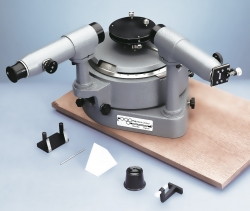
\includegraphics[width=0.45\textwidth]{goniometer}
	\caption{Goniómetro de Babinet (modelo Philipe Harris Advanced Spectrometer 30). \label{fig:goniometer}} 
\end{figure}

O colimador é constituído por dois tubos cilíndricos concêntricos que se podem deslocar axialmente. Um deles possui uma fenda retilínea, de largura variável por um parafuso, e que deve ser colocada na vertical (pode utilizar a mira da ocular depois de regulada). O outro tubo tem no extremo oposto (mais próximo do eixo) uma lente convergente, $L_C$. O objetivo deste conjunto, quando a fenda é iluminada por uma fonte luminosa divergente, é produzir um feixe de raios paralelos na região da plataforma, onde se coloca o prisma, rede, ou espelho. A fenda, se for relativamente estreita, vai funcionar como objeto linear.

\begin{figure}[!htb]  
	\centering 
	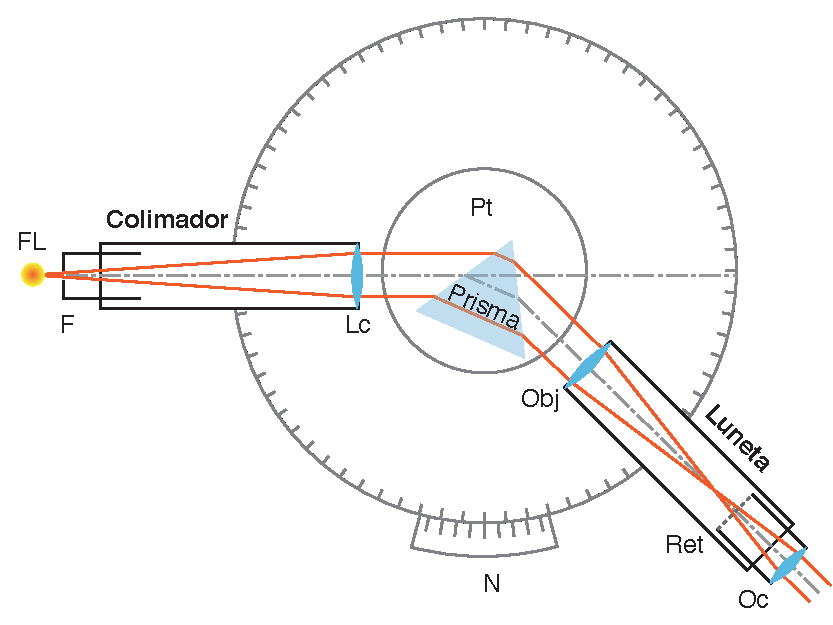
\includegraphics[width=0.65\textwidth]{Babinet}
	\caption{Esquema do Goniómetro de Babinet. Legenda: FL -- fonte luminosa, F -- fenda, Lc -- lente convergente do colimador, Pt -- plataforma, Obj -- objetiva, Oc -- ocular, Ret -- retículo, N -- nónio acoplado à luneta\label{fig:babinet}} 
\end{figure}

A luneta é constituída por dois elementos ópticos, uma lente convergente e uma ocular munida de retículo (dois fios cruzados perpendicularmente). A primeira lente produz no seu plano focal a imagem intemédia da fenda, que é projetada no plano do retículo e ampliada pela ocular. A ocular é regulada pelo observador, de modo a ver uma imagem focada da fenda. Quando se dispõe de um sistema de deteção (placa fotográfica ou um detetor, por exemplo uma célula fotoelétrica com um sistema de amplificação), este é colocado diretamente no plano focal da lente convergente e é retirada a ocular.
A regulação do instrumento pelo utilizador é feita sempre na seguinte ordem:
\begin{enumerate}
\item Focar  o retículo para um olho sem necessidade de acomodação (relaxado) e alinhá-lo com a vertical usando um fio de prumo, ou alguma linha vertical no laboratório.
\item Focar a ocular observando um objecto no infinito (ou quase).
\item Alinhar a luneta e o colimador para observar a fenda iluminada. Focar a imagem da fenda, regulando APENAS o parafuso do colimador.
\item Alinhar a fenda com a vertical, sobrepondo a mira e reduzir a sua largura para um valor suficientemente estreito, embora claramente visível.
\end{enumerate}

\subsection{\sf Procedimento experimental}
%\subsection{\sf Questões a responder ANTES da sessão de Laboratório:}
%\begin{enumerate}
%\item Descreva por palavras suas quais os objectivos do Trabalho que irá realizar na sessão de Laboratório (uma folha A4). Indique as expressões que irá utilizar para obter as grandezas experimentais, bem como as expressões para calcular as incertezas. Inclua esta parte também no Relatório. Este irá constituir o ÚNICO meio de consulta na Prova Individual.
	
%\item A partir da equação das lentes delgadas $\frac{1}{f} = (n_{vidro}-1) \left(\frac{1}{R_1} -\frac{1}{R_2}\right)$ e assumindo que os dois raios $R_1$ e $R_2$ das superfícies esféricas das lentes utilizadas no trabalho anterior são iguais e $ n_{vidro}=1.57$, calcule $R_{1,2}$ para todas as lentes esféricas utilizadas no trabalho de Ótica.
%\item Assumindo que o diâmetro das lentes é $D=4$ cm, calcule a sua espessura mínima. Podem ser fielmente consideradas como lentes delgadas?
%\item Como variam as distâncias focais se estas lentes forem mergulhada em água? (\emph{Sugestão: considere a forma da equação das lentes delgadas.})
%\end{enumerate}

Material utilizado
%1ª Parte
%\begin{itemize}
%\item caixa de ótica equipada com calha graduada
%\item lentes convergentes e divergente
%\item semi-cilindro de vidro acrílico
%\item objeto com mira
%\item diafragmas
%\item suportes
%\item fonte luminosa com lâmpada de incandescência linear
%\end{itemize}

%2ª Parte
\begin{itemize}
\item goniómetro
\item fonte de luz incandescente (candeeiro)
\item luz espetral de Hg ou He
\item prisma
\item rede de difração
\item nível graduado
\end{itemize}

%\subsection{\sf Procedimento Experimental}

%\subsubsection{\sf  Telescópio}

%A montagem  a utilizar é da Figura \ref{fig:Telescopio}, embora o objecto esteja situado a uma distância grande (> 5 m). 

%\begin{enumerate}
%\item Na folha quadriculada em anexo desenhe um diagrama de traçado de raios, utilizando como objectiva a lente mais potente do trabalho de Ótica Geométrica, e considerando o objecto no infinito. Obtenha a posição da imagem intermédia (plano focal). 
%\item Calcule agora a posição da lente ocular, com $f_{ocu}=150$ mm, para obter uma ampliação transversal entre a imagem intermédia e a imagem final de $M_T=-3$. 
%\item Utilizando as aproximações paraxial e das lentes delgadas, desenhe a construção geométrica e obtenha a posição da imagem e a respetiva ampliação.
%\item Tente montar o sistema na calha e observe um objeto distante a partir da lente ocular. Foque bem a imagem e registe a posição das duas lentes. Compare com o diagrama de traçado de raios.
%\item Calcule a o Número f do telecópio (inverso da Abertura %relativa)   a partir dos diâmetro, $D$, e distancia focal da %Objetiva, $f$. Compare com o valores das máquinas fotográficas %comerciais.
%$$f/\# \equiv \frac{}{}$$. 
%\end{enumerate}

%\subsubsection{\sf  Microscópio}

%Nesta montagem equivalente, iremos trocar a posição da lentes (objetiva/ocular) e colocar um pequeno objeto a uma distância um pouco maior que a distância focal da objetiva $f_{obj}$. A ampliação total deste sistema é o produto da ampliação transversal da objectiva, $M_{T_{obj}}$,  e da \emph{ampliação angular}\footnote{Definida como a razão entre a dimensão da imagem na retina quando o objeto é visto através da lente e a dimensão do objecto quando visto pelo olho desarmado à distância normal de observação, que é cerca de 25 cm.} da ocular, $M_{A_{ocu}}$.
 
%A ampliação transversal é calculada pela razão
%$$M_{T_{obj}}=-\frac{d_I}{d_O}=-\frac{d_I - f_{obj}}{f_{obj}}$$

%A ampliação angular pode ser estimada por 
%$$M_{A_{ocu}}= \frac{0.25}{f_{ocu}}$$

%\begin{enumerate}
%\item Na folha quadriculada em anexo desenhe um diagrama de traçado de raios, com o objecto a uma distância do foco igual $\approx f/5$. Obtenha a posição da imagem intermédia. Calcule agora a posição da lente ocular para obter um feixe de raios paralelos (imagem no infinito).
%\item Tente montar o sistema na calha e observe o slide com a mira graduada. Com auxílio do slide transparente graduado, tente estimar a ampliação do  objeto distante a partir da lente ocular. Foque bem a imagem e registe a posição das duas lentes. Compare com o diagrama de traçado de raios.
%\item Calcule a ampliação total do sistema.
%\item Identifique os vários tipos de imperfeição que pode observar na imagem. 
%\end{enumerate}

%\subsubsection{\sf Goniómetro de Babinet}

Procedimento
\begin{enumerate}
%\item Ligue  a  lâmpada  espetral  e  espere  10  a  15  minutos    %até  que  se  estabeleça  o 
%equilíbrio térmico no seu interior. 
\item Disponha o goniómetro em frente a uma fonte luminosa de luz incandescente.
\item Comece por regular a ocular da luneta do goniómetro. Para isso deve ver nitidamente com um 
olho  os fios do retículo, e simultaneamente com o outro olho ver um objeto no exterior da luneta afastado a cerca de 30 cm.  
\item Para  regular  a  objetiva,  observe  agora  um  objeto  no  “infinito” (no  laboratório 
escolha  um objeto  mais  afastado possível)  atuando  sobre  o  parafuso  da  luneta.  Regule  de  modo  a 
observar o objeto e o retículo bem focado e sem paralaxe. 
\item Coloque  a  luneta  alinhada de frente  do  colimador  e  regule o parafuso  do 
colimador de modo a observar a fenda focada quando iluminada pela lâmpada espetral. 
\item Com a ajuda do nível de bolha, verifique o nivelamento horizontal do goniómetro e da plataforma onde vai colocar o prisma.
\item Identifique as escalas dos ângulos, para medir a posição da plataforma e da luneta. Como estão relacionadas as duas escalas opostas. Qual a resolução mínima do conjunto escala/nónio?
\item Observe a reflexão em cada face que define o ângulo do prisma e registe a posição angular 
correspondente a essas reflexões. Cada observador deve fazer uma determinação usando o 
parafuso  micrométrico e centrando  a  imagem  da  fenda  com  o retículo  por  aproximação  à direita e à esquerda. Calcule o ângulo principal entre as duas faces polidas do prisma através desta medição.
\item Substitua no centro da plataforma do goniómetro o prisma por uma rede de difração de 
600 linhas por milímetro, e a fonte por uma luz espectral (lâmpada de mercúrio ou hélio). Observe os raios \emph{difratados} de várias cores, em 1.ª e 2.ª ordem. Tente medir os ângulos de desvio, com a melhor precisão possível.

\end{enumerate}


	
\newpage
\def\width{18}
\def\hauteur{25}
\begin{tikzpicture}[x=1cm, y=1cm, semitransparent]
\draw[step=1mm, line width=0.1mm, black!30!white] (0,0) grid (\width,\hauteur);
\draw[step=5mm, line width=0.2mm, black!40!white] (0,0) grid (\width,\hauteur);
\draw[step=5cm, line width=0.5mm, black!50!white] (0,0) grid (\width,\hauteur);
\draw[step=1cm, line width=0.3mm, black!90!white] (0,0) grid (\width,\hauteur);
\end{tikzpicture}

\newpage
\def\width{18}
\def\hauteur{25}
\begin{tikzpicture}[x=1cm, y=1cm, semitransparent]
\draw[step=1mm, line width=0.1mm, black!30!white] (0,0) grid (\width,\hauteur);
\draw[step=5mm, line width=0.2mm, black!40!white] (0,0) grid (\width,\hauteur);
\draw[step=5cm, line width=0.5mm, black!50!white] (0,0) grid (\width,\hauteur);
\draw[step=1cm, line width=0.3mm, black!90!white] (0,0) grid (\width,\hauteur);
\end{tikzpicture}

\end{document} 